%Dokument pro XeLaTeX, překlad pomocí XeLaTeX
\documentclass[a4paper,oneside,11pt,usenames,dvipsnames]{article}

%XeLaTeXové věci a fonty
\usepackage{fontspec,xltxtra,xunicode}
\defaultfontfeatures{Scale=MatchLowercase}

%Písma
%\setromanfont[Mapping=tex-text]{Linux Libertine O}
%\setsansfont[Mapping=tex-text]{Linux Biolinum O}
%\setmonofont[Mapping=tex-text]{Linux Libertine Mono O}

%Pro správné dělení českých slov
\usepackage{polyglossia}
\setdefaultlanguage{czech} %TODO: Případně změňte jazyk
%České uvozovky buď přímo nebo jako ,,uvozovky``

%Některé speciální znaky
\usepackage{textcomp}
% Url
\usepackage{url}
\def\UrlFont{\ttfamily\slshape}

%Barvy pro hyperref
\usepackage{color}
% Hyperref pro odkazy v PDF a URL
\usepackage{hyperref}


\usepackage{lmodern}
\usepackage{geometry}
\geometry{margin=2.5cm}
\usepackage{graphicx}
\usepackage{booktabs}
\usepackage{amsmath}

% Hyperref a PDF nastavení
\hypersetup{
    pdftitle={Seminární práce: Keras a TensorFlow},    % title TODO: Vyplnit titulek
    pdfauthor={Ondřej Maxa},     % author TODO: Vyplnit autora
    colorlinks=true,       % false: boxed links; true: colored links
    linkcolor=RoyalBlue,          % color of internal links
    citecolor=RoyalBlue,        % color of links to bibliography
    filecolor=RoyalBlue,      % color of file links
    urlcolor=RoyalBlue           % color of external links
}

%Nadpisy, záhlaví a zápatí
\usepackage[pagestyles]{titlesec}

%Nadpisy bezpatkovým písmem
\titleformat{\part}[display]{\filright}{\Large\sffamily Část\ \thepart}{0.25em}{\bfseries\sffamily\huge\upshape}
\titleformat{\section}[block]{\sffamily\Large\bfseries}{\thesection}{1em}{\Large}
\titleformat{\subsection}[block]{\sffamily\large\bfseries}{\thesubsection}{1em}{\large}
\titleformat{\subsubsection}[block]{\sffamily\normalsize\bfseries}{\thesubsubsection}{1em}{\normalsize}

\begin{document}

\thispagestyle{empty}
\begin {center}
	\vspace *{10mm}
	{\Huge \sffamily \bfseries Seminární práce: Keras a TensorFlow}

	\vspace *{20mm}
	{\Large \sffamily \bfseries Ondřej Maxa}

	\vspace *{7.5mm}
	{\large \sffamily 16. prosince 2025}
\end {center}

\begin{abstract}
	Tato seminární práce se zabývá využitím frameworků TensorFlow a Keras pro úlohu binární analýzy sentimentu krátkých produktových recenzí z datasetu Sentiment Labelled Sentences -- Amazon \cite{uci_sls}. Cílem práce je ukázat kompletní postup od předzpracování textu přes návrh architektury neuronové sítě až po experimentální vyhodnocení různých konfigurací modelu. Pro reprezentaci textu je použita vrstva \texttt{TextVectorization} a embedding, nad nimiž jsou testovány jak jednoduché husté modely, tak konvoluční architektura s vrstvou \texttt{Conv1D}. Výsledky ukazují, že vhodně navržený konvoluční model dosahuje validační přesnosti přibližně 80\,\% a překonává jednodušší konfigurace z hlediska generalizace na validační množinu.
\end{abstract}

\setlength{\parskip}{1ex plus 0.25ex minus 0.125ex}
  
\section{Úvod}
\label{sec:uvod}
V posledních letech se metody hlubokého učení staly standardním nástrojem pro řešení úloh zpracování přirozeného jazyka, jako je strojový překlad, sumarizace či analýza sentimentu zákaznických recenzí. Framework TensorFlow a jeho vysokourovňové API Keras umožňují relativně snadno navrhovat, trénovat a vyhodnocovat neuronové sítě i uživatelům, kteří nejsou odborníky na nízkoúrovňovou implementaci numerických výpočtů. Cílem této seminární práce je na jednoduchém datasetu sentimentu ukázat celý proces vytvoření modelu v Kerasu nad TensorFlow, od předzpracování dat přes návrh architektury až po experimentální porovnání různých konfigurací.

Pro experimenty je použit dataset \emph{Sentiment Labelled Sentences -- Amazon}, který obsahuje krátké textové recenze produktů z internetového obchodu Amazon. Každá věta je anotována binárním štítkem 0 nebo 1, což označuje negativní, respektive pozitivní sentiment. Úlohu lze tedy formulovat jako binární klasifikaci, kde vstupem je věta v angličtině a výstupem pravděpodobnost, že recenze vyjadřuje pozitivní hodnocení. Hlavní výzkumná otázka této práce zní: jaký vliv mají různé architektury neuronové sítě a trénovací hyperparametry na přesnost modelu sentiment analýzy při použití Kerasu a TensorFlow.
 
\section{Metody}
\label{sec:metody}

\subsection{Data a předzpracování}
\label{subsec:data-a-predzpracovani}
Dataset \texttt{amazon\_cells\_labelled.txt} obsahuje 1000 vět, každou na jednom řádku ve tvaru ``věta<TAB>label''. Textová část byla načtena do datového rámce jazyka Python, náhodně promíchána a rozdělena na tři části: 70\,\% záznamů pro trénovací sadu, 15\,\% pro validační a 15\,\% pro testovací sadu, aby bylo možné model ladit a zároveň objektivně vyhodnotit jeho zobecňovací schopnost.

Pro převod textu na číselnou reprezentaci byla použita vrstva \texttt{TextVectorization} z Kerasu, která nejprve vytvořila slovník nejvýše 10\,000 nejčastějších tokenů v trénovací sadě. Každá věta byla převedena na sekvenci celých čísel, kde každé číslo reprezentuje jeden token, a sekvence byly zkráceny nebo doplněny (padding) na maximální délku 40 tokenů, aby měly všechny vstupy stejný tvar vhodný pro vstup do neuronové sítě. Takto vektorizovaná data byla dále zabalena do objektů \texttt{tf.data.Dataset}, které umožňují efektivní dávkování (batching) a přednačítání (prefetching) během trénování.

\subsection{Základní architektura modelu}
\label{subsec:zakladni-architektura-modelu}
Jako referenční architektura byl zvolen model složený z embedding vrstvy, pooling vrstvy a jedné skryté husté (Dense) vrstvy. Embedding vrstva převádí indexy tokenů na husté vektory délky 64, čímž umožňuje modelu naučit se distribuované reprezentace slov. Nad výstupem embeddingu je použita buď globální průměrovací poolingová vrstva, nebo konvoluční vrstva s jednorozměrnou konvolucí, jak je popsáno níže. Skrytá vrstva \texttt{Dense(64)} používá jako aktivační funkci ReLU a výstupní vrstva \texttt{Dense(1)} používá sigmoid pro výpočet pravděpodobnosti kladného sentimentu.

Model byl kompilován s optimalizační metodou Adam, ztrátovou funkcí \texttt{binary\_crossentropy} a metrikou přesnosti (\texttt{accuracy}). Trénování probíhalo v několika bězích, přičemž v každém experimentu se měnila vždy jen jedna skupina parametrů -- počet epoch, velikost dávky, počet vrstev, typ aktivačních funkcí, ztrátových funkcí nebo optimalizátorů. Pro každou konfiguraci byly uloženy trénovací a validační křivky ztráty a přesnosti, které jsou shrnuty v~tabulce~\ref{tab:configs} a na obrázcích v části Výsledky.

\subsection{Konfigurace modelu C\label{subsec:konfigurace-modelu-c}}
Nejlepšího výkonu dosáhl model označený jako \emph{model C}, jehož architektura kombinuje embedding, konvoluční vrstvu a pooling. Konkrétně má tvar:
\begin{itemize}
    \item \texttt{Embedding(input\_dim=10000, output\_dim=64, input\_length=40)}
    \item \texttt{Conv1D(64, kernel\_size=3, activation="relu")}
    \item \texttt{GlobalMaxPooling1D()}
    \item \texttt{Dense(64, activation="relu")}
    \item \texttt{Dropout(0.5)}
    \item \texttt{Dense(1, activation="sigmoid")}
\end{itemize}
Tento model byl trénován 10 epochami s batch size 32, optimizérem Adam, ztrátovou funkcí \texttt{binary\_crossentropy} a výše popsaným předzpracováním textu. Pro porovnání byly vyzkoušeny i jednodušší modely (pouze pooling + výstupní vrstva) a složitější vícevrstvé varianty, stejně jako alternativní aktivační funkce (tanh), ztrátová funkce hinge a optimalizátory SGD s momentum a RMSprop.

\subsection{Přehled konfigurací\label{subsec:prehled-konfiguraci}}
Shrnutí hlavních konfigurací a jejich výsledků na validační sadě je uvedeno v tabulce~\ref{tab:configs}. Hodnoty vycházejí z automatizovaných běhů, jejichž křivky trénování jsou uloženy v obrázcích \texttt{./images/\{name\}\_loss.png} a \texttt{./images/\{name\}\_accuracy.png}.

\begin{table}[ht]
\centering
\caption{Přehled testovaných konfigurací modelu a jejich výsledků na testovací sadě.\label{tab:configs}}
\begin{tabular}{@{}l|cc|r@{}}
\toprule
Jméno běhu & Ztráta (test\_loss) & Přesnost (test\_acc) & Čas běhu \\
\midrule
default    & 0.569 & 0.753 & 8.45s \\
5-epochs   & 0.681 & 0.540 & 5.82s \\
20-epochs  & 0.455 & 0.773 & 12.92s \\
16-batches & 0.437 & 0.800 & 11.51s \\
64-batches & 0.654 & 0.680 & 7.04s \\
model\_a   & 0.671 & 0.600 & 7.93s \\
model\_c   & 0.432 & 0.787 & 8.53s \\
1d\_cnn    & 0.398 & 0.807 & 9.65s \\
tanh       & 0.525 & 0.753 & 8.40s \\
hinge      & 1.012 & 0.473 & 7.69s \\
sgd        & 0.696 & 0.473 & 5.47s \\
rmsprop    & 0.693 & 0.473 & 6.71s \\
\bottomrule
\end{tabular}
\end{table}

\section{Výsledky}
\label{sec:vysledky}

\subsection{Počet epoch a velikost dávky}
\label{subsec:pocet-epoch-a-velikost-davky}
Změna počtu epoch ukázala, že model potřebuje alespoň přibližně deset průchodů nad trénovací sadou, aby dosáhl dobrého výkonu na validačních datech. Při trénování pouze pět epoch skončila validační přesnost okolo 47\,\% a validační ztráta se snižovala jen velmi pomalu, což odpovídá podučenému modelu, který ještě nenašel vhodnou reprezentaci (viz obr.~\ref{fig:5epochs-loss} a \ref{fig:5epochs-acc}). Naopak dvacet epoch vedlo k podobné validační přesnosti jako deset epoch, ale s výrazně nižší trénovací ztrátou a rostoucím rozdílem mezi trénovací a validační chybou po dvanácté epoše, což je náznak přeučení (obr.~\ref{fig:20epochs-loss} a \ref{fig:20epochs-acc}).

Velikost dávky měla rovněž znatelný vliv. Základní nastavení 32 dosahovalo validační přesnosti přibližně 76\,\%, zatímco menší batch 16 tuto hodnotu mírně zlepšil na přibližně 77--78\,\%. Naproti tomu větší batch 64 vedl k poklesu validační přesnosti na zhruba 63\,\% a vyšší ztrátě, což potvrzuje, že příliš velké dávky mohou zhoršit schopnost modelu generalizovat na nové příklady. Tyto rozdíly jsou dobře patrné na křivkách v obr.~\ref{fig:16batches-loss}--\ref{fig:64batches-acc}.

\subsection{Vliv architektury}
\label{subsec:vliv-architektury}
Porovnání jednoduchého modelu A, referenčního modelu B (default) a složitějšího modelu C ukázalo, že architektura má pro sentiment analýzu zásadní význam. Model A, který používá pouze embedding následovaný poolingem a výstupní jednotkou se sigmoid aktivací, dosáhl validační přesnosti zhruba 59\,\% a relativně vysoké ztráty, což naznačuje, že jeho kapacita je pro danou úlohu nedostatečná. Model B s jednou skrytou vrstvou Dense(64) představuje výrazné zlepšení a dosahuje validační přesnosti kolem 76\,\%.

Nejlepších výsledků dosáhl model C, který kombinuje konvoluční vrstvu Conv1D, globální max-pooling a hustou vrstvu s 64 neurony. Tento model dosáhl validační přesnosti přibližně 80\,\% a nejnižší validační ztráty ze všech testovaných konfigurací, jak ukazují grafy na obr.~\ref{fig:modelc-loss} a \ref{fig:modelc-acc}.

\subsection{Aktivační funkce, ztráta a optimalizátory}
\label{subsec:aktivacni-funkce-ztrata-a-optimalizatory}
Experiment s aktivační funkcí tanh ukázal, že nahrazení ReLU ve skrytých vrstvách nevede k dramatické změně výkonu: validační přesnost zůstala blízko 76\,\%, zatímco ztráta se mírně snížila, jak je patrné z obr.~\ref{fig:tanh-loss} a \ref{fig:tanh-acc}. Výrazně horších výsledků bylo dosaženo se ztrátovou funkcí hinge: validační přesnost klesla na přibližně 46\,\% a ztráta byla několikanásobně vyšší, což potvrzuje, že pro binární sentiment analýzu s pravděpodobnostním výstupem je vhodnější \texttt{binary\_crossentropy} (obr.~\ref{fig:hinge-loss} a \ref{fig:hinge-acc}).

Porovnání optimalizačních algoritmů potvrdilo, že Adam je pro tuto úlohu nejefektivnější volbou. Běhy se SGD s momentum i s RMSprop skončily na validační přesnosti kolem 47\,\% a se ztrátou okolo 0{,}69, tedy prakticky na úrovni náhodného hádání, jak ukazují grafy na obr.~\ref{fig:sgd-loss} a na obr.~\ref{fig:sgd-acc}.

\section{Diskuse a závěr}
Výsledky experimentů ukazují, že i na relativně malém datasetu o velikosti 1000 vět umožňuje použití Kerasu a TensorFlow poměrně snadno navrhnout a vyhodnotit různé architektury pro sentiment analýzu. Přitom se potvrzuje několik obecných poznatků z hlubokého učení: model musí mít dostatečnou kapacitu, ale nesmí být zbytečně složitý vzhledem k množství dat, je potřeba pečlivě volit počet epoch a velikost dávky a zásadní je i volba vhodné ztrátové funkce a optimalizátoru.

Nejlepší zkoumaný model C, tvořený embeddingem, konvoluční vrstvou, globálním max-poolingem, hustou vrstvou s ReLU a výstupem se sigmoid aktivací, dosáhl validační přesnosti okolo 80\,\%, což lze pro jednoduchý dataset krátkých recenzí považovat za uspokojivý výsledek. Další zlepšení by pravděpodobně přineslo použití většího trénovacího korpusu, předtrénovaných embeddingů nebo modernějších architektur typu Transformer; tyto možnosti však přesahují rámec této seminární práce.

Z hlediska praktické práce s Kerasem a TensorFlow byla nejdůležitější zkušeností jednoduchost definice modelu v podobě sekvenčního seznamu vrstev a možnost systematicky měnit jednotlivé hyperparametry bez zásahu do zbytku kódu. Experimenty s různými konfiguracemi zároveň ukázaly, jak důležité je průběžné sledování validační ztráty a použití strategií jako \emph{early stopping}, aby se předešlo zbytečně dlouhému trénování a přeučení. Celkově lze říci, že použití Kerasu nad TensorFlow poskytuje vhodný nástroj pro výukové projekty v oblasti umělé inteligence a umožňuje studentům soustředit se na koncepční návrh modelu a interpretaci výsledků namísto řešení implementačních detailů numerických výpočtů.

\begin{thebibliography}{11}
\setlength{\parskip}{0ex}

	\bibitem{uci_sls}
	Github: Microsoft - ML-Server-Python-Samples. \textless\url{https://github.com/microsoft/ML-Server-Python-Samples/blob/master/microsoftml/202/data/sentiment_analysis/amazon_cells_labelled.txt}\textgreater.

	\bibitem{tf_text}
	TensorFlow Tutorials: Basic text classification. \textless\url{https://www.tensorflow.org/tutorials/keras/text_classification}\textgreater.

	\bibitem{keras_example}
	Keras Examples: Text classification from scratch. \textless\url{https://keras.io/examples/nlp/text_classification_from_scratch/}\textgreater.

	\bibitem{keras_opt}
	TensorFlow Guide: Optimizers. \textless\url{https://www.tensorflow.org/api_docs/python/tf/keras/optimizers}\textgreater.

\end{thebibliography}

\appendix
\section*{Přílohy}

\begin{figure}[ht!]
    \centering
    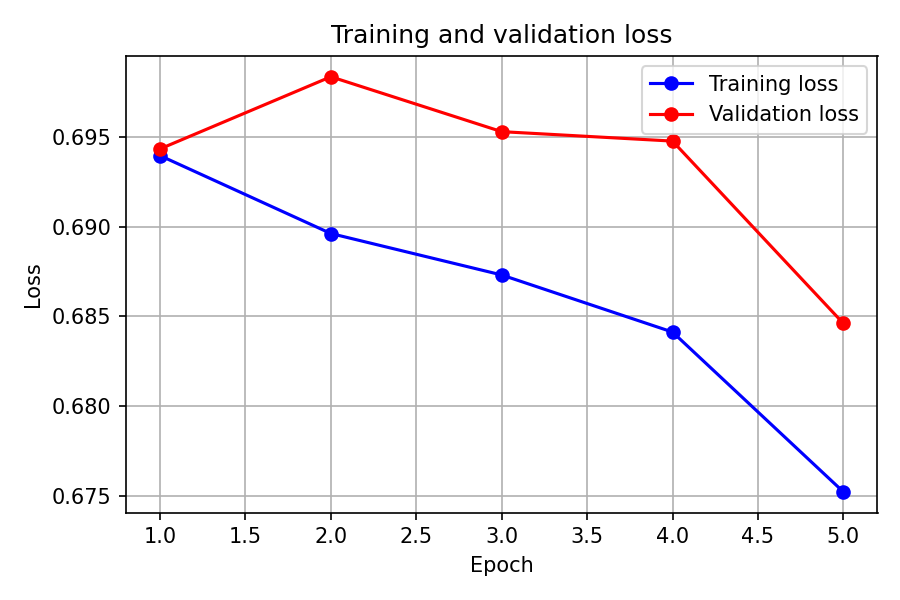
\includegraphics[width=1.0\linewidth]{./images/5-epochs_loss.png}
    \caption{Průběh trénovací a validační ztráty pro konfiguraci \texttt{5-epochs}, která ukazuje podučení modelu po pěti epochách.\label{fig:5epochs-loss}}
\end{figure}

\begin{figure}[ht!]
    \centering
    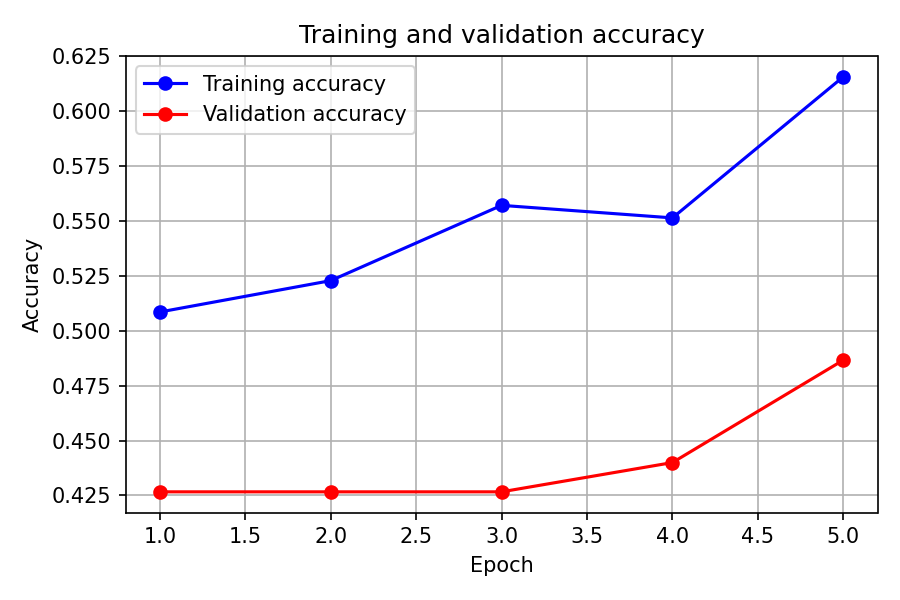
\includegraphics[width=1.0\linewidth]{./images/5-epochs_accuracy.png}
    \caption{Trénovací a validační přesnost pro konfiguraci \texttt{5-epochs}, kde validační přesnost zůstává nízká.\label{fig:5epochs-acc}}
\end{figure}

\begin{figure}[ht!]
    \centering
    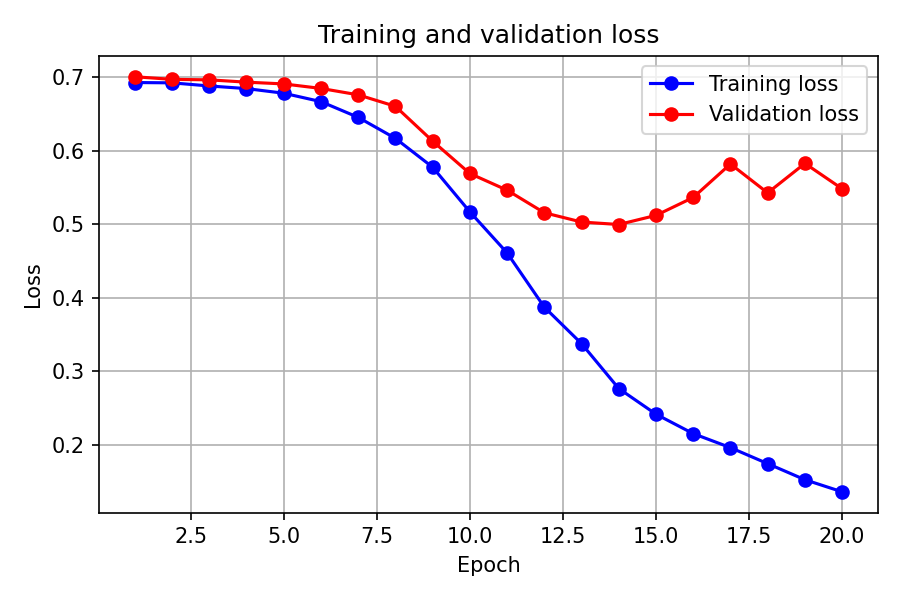
\includegraphics[width=1.0\linewidth]{./images/20-epochs_loss.png}
    \caption{Průběh ztráty pro konfiguraci \texttt{20-epochs}; po přibližně 12 epochách je patrný náznak přeučení podle chování validační ztráty.\label{fig:20epochs-loss}}
\end{figure}

\begin{figure}[ht!]
    \centering
    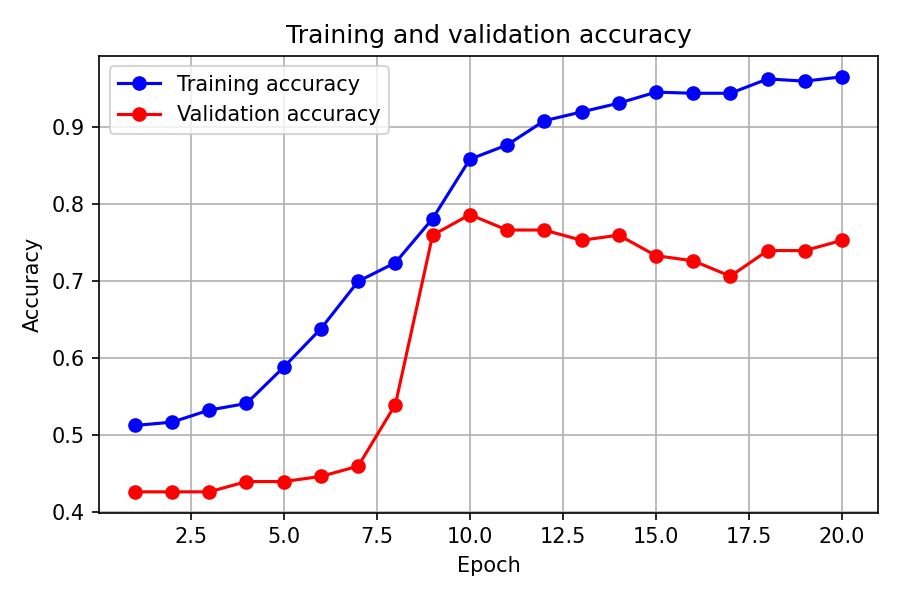
\includegraphics[width=1.0\linewidth]{./images/20-epochs_accuracy.png}
    \caption{Trénovací a validační přesnost pro konfiguraci \texttt{20-epochs}; přesnost na trénovacích datech roste, zatímco validační se stabilizuje.\label{fig:20epochs-acc}}
\end{figure}

\begin{figure}[ht!]
    \centering
    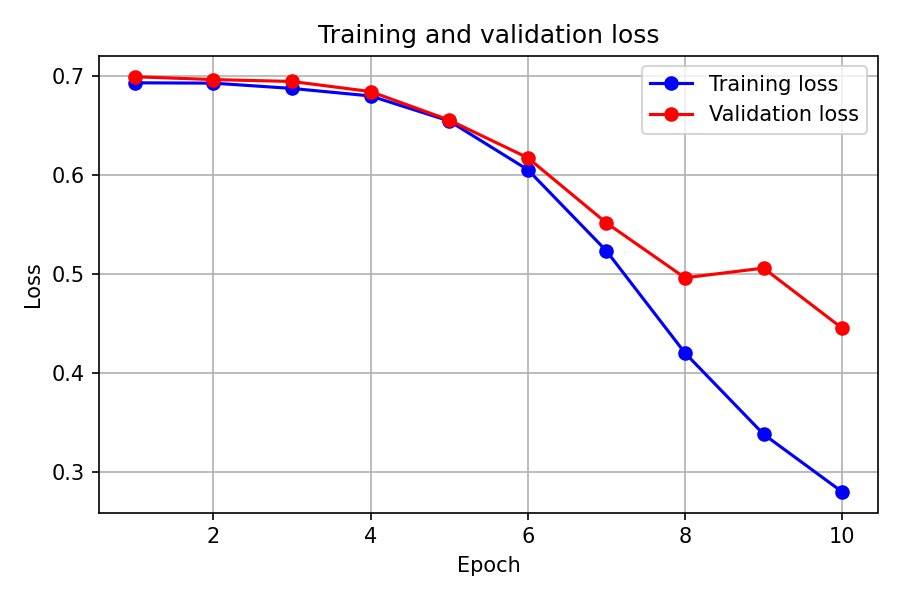
\includegraphics[width=1.0\linewidth]{./images/16-batches_loss.png}
    \caption{Průběh ztráty pro konfiguraci s menší dávkou \texttt{16-batches}; validační ztráta je nižší než u defaultní konfigurace.\label{fig:16batches-loss}}
\end{figure}

\begin{figure}[ht!]
    \centering
    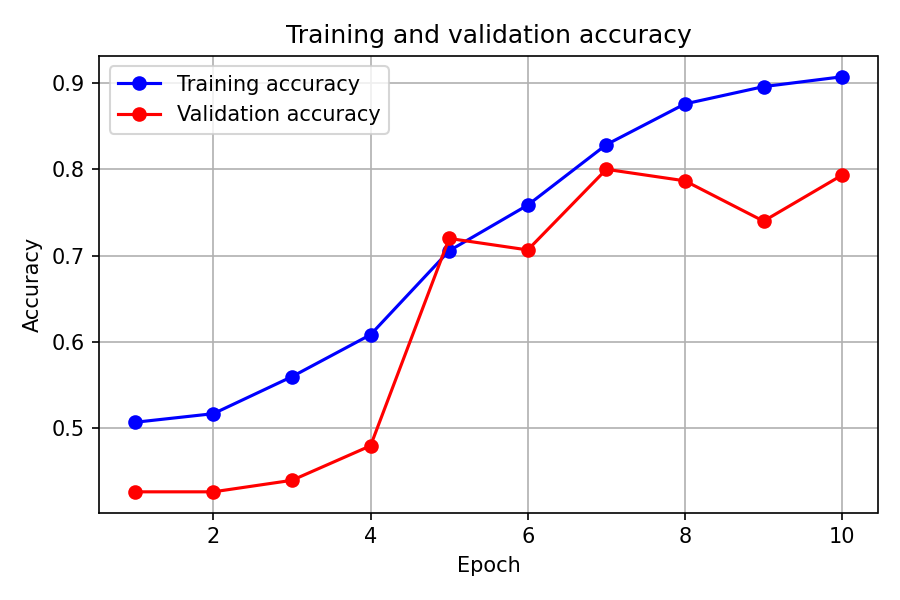
\includegraphics[width=1.0\linewidth]{./images/16-batches_accuracy.png}
    \caption{Přesnost pro konfiguraci \texttt{16-batches}, která dosahuje mírně lepší generalizace než výchozí nastavení.\label{fig:16batches-acc}}
\end{figure}

\begin{figure}[ht!]
    \centering
    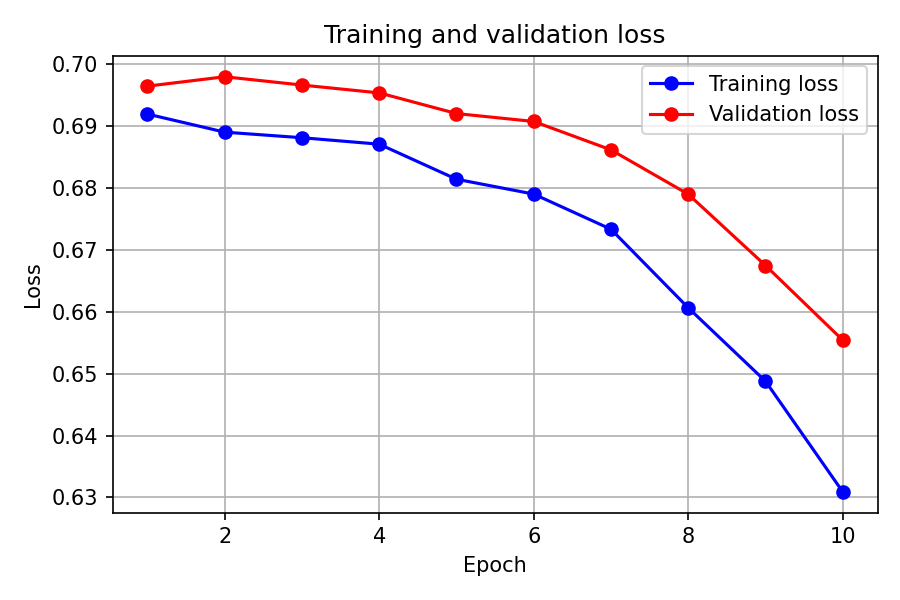
\includegraphics[width=1.0\linewidth]{./images/64-batches_loss.png}
    \caption{Ztráta pro konfiguraci \texttt{64-batches}; vyšší dávka vede k horší validační ztrátě.\label{fig:64batches-loss}}
\end{figure}

\begin{figure}[ht!]
    \centering
    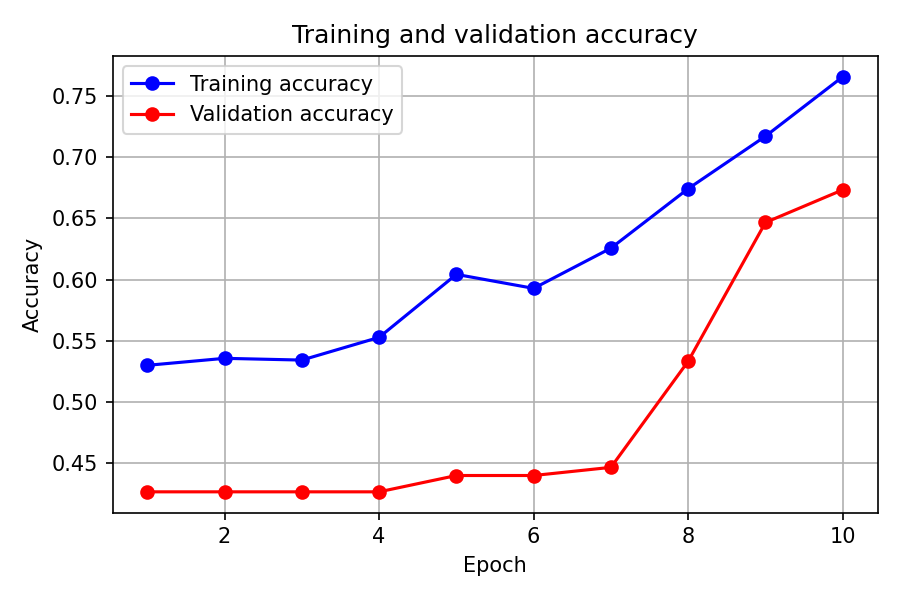
\includegraphics[width=1.0\linewidth]{./images/64-batches_accuracy.png}
    \caption{Přesnost pro konfiguraci \texttt{64-batches}, kde model dosahuje nejnižší validační přesnosti.\label{fig:64batches-acc}}
\end{figure}

\begin{figure}[ht!]
    \centering
    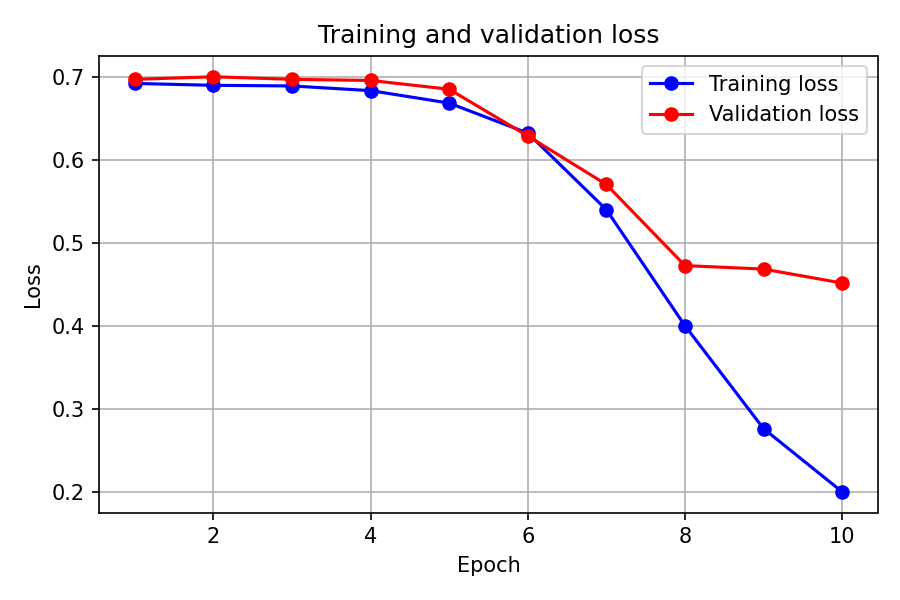
\includegraphics[width=1.0\linewidth]{./images/model_c_loss.png}
    \caption{Průběh ztráty pro nejlepší konfiguraci \texttt{model\_c} s konvoluční architekturou.\label{fig:modelc-loss}}
\end{figure}

\begin{figure}[ht!]
    \centering
    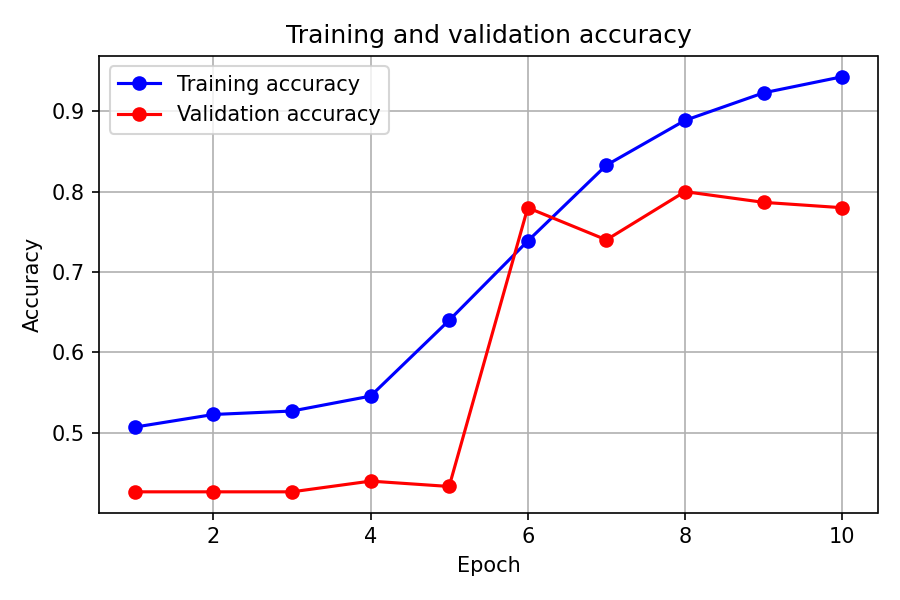
\includegraphics[width=1.0\linewidth]{./images/model_c_accuracy.png}
    \caption{Přesnost na trénovací a validační sadě pro konfiguraci \texttt{model\_c}, která dosahuje nejvyšší validační přesnosti.\label{fig:modelc-acc}}
\end{figure}

\begin{figure}[ht!]
    \centering
    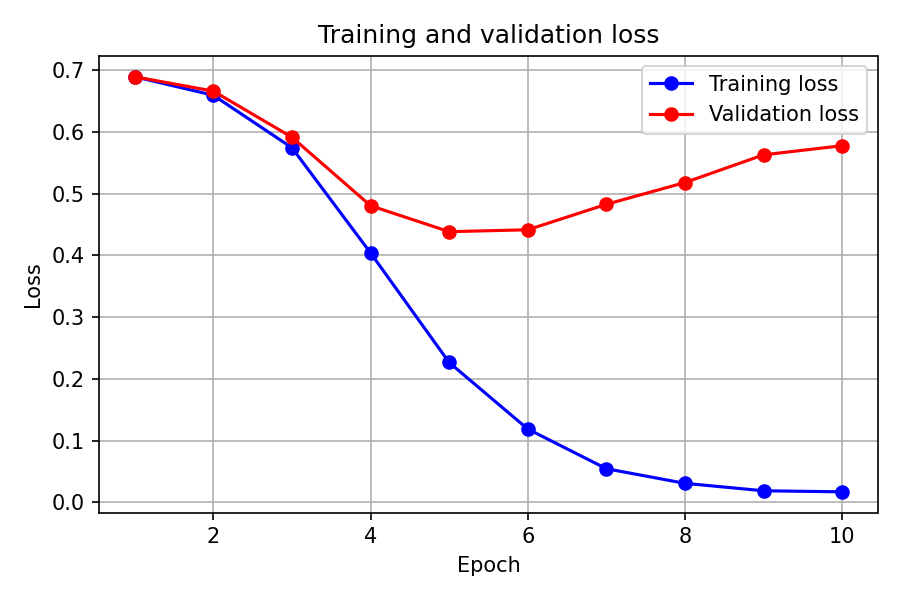
\includegraphics[width=1.0\linewidth]{./images/1d_cnn_loss.png}
    \caption{Průběh ztráty pro nejlepší konfiguraci \texttt{1d\_cnn} s konvoluční architekturou.\label{fig:1dcnn-loss}}
\end{figure}

\begin{figure}[ht!]
    \centering
    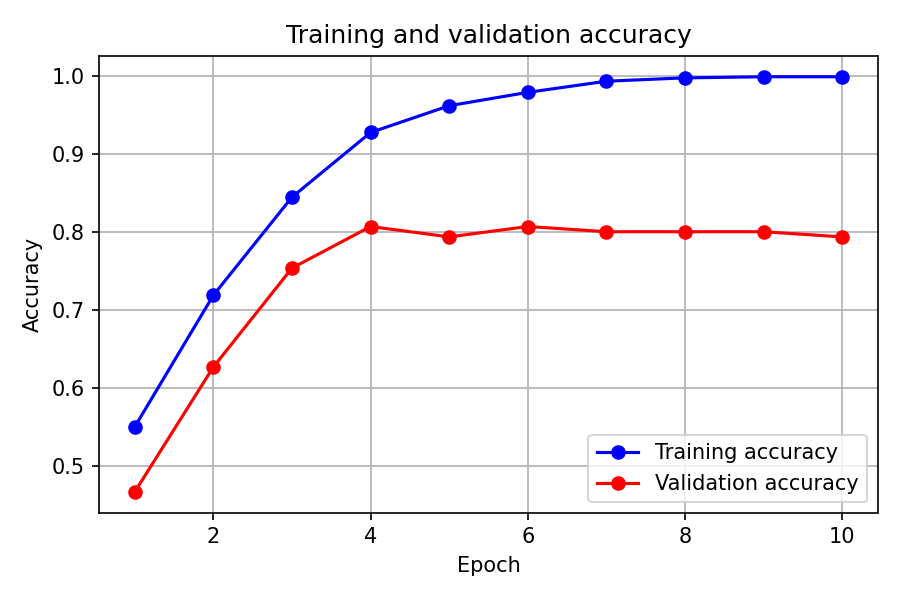
\includegraphics[width=1.0\linewidth]{./images/1d_cnn_accuracy.png}
    \caption{Přesnost na trénovací a validační sadě pro konfiguraci \texttt{1d\_cnn}, která dosahuje nejvyšší validační přesnosti.\label{fig:1dcnn-acc}}
\end{figure}

\begin{figure}[ht!]
    \centering
    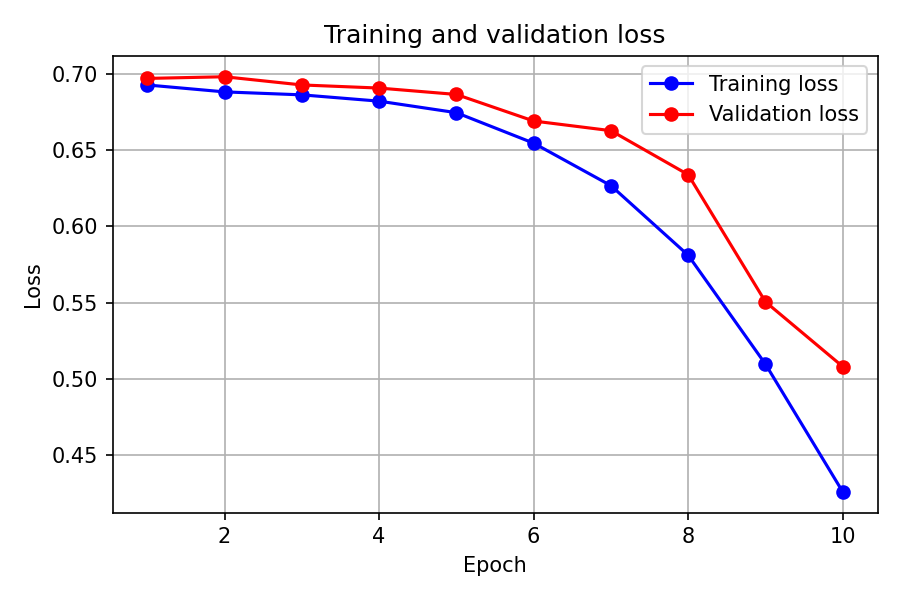
\includegraphics[width=1.0\linewidth]{./images/tanh_loss.png}
    \caption{Ztráta pro konfiguraci \texttt{tanh} se skrytými vrstvami s aktivační funkcí tanh.\label{fig:tanh-loss}}
\end{figure}

\begin{figure}[ht!]
    \centering
    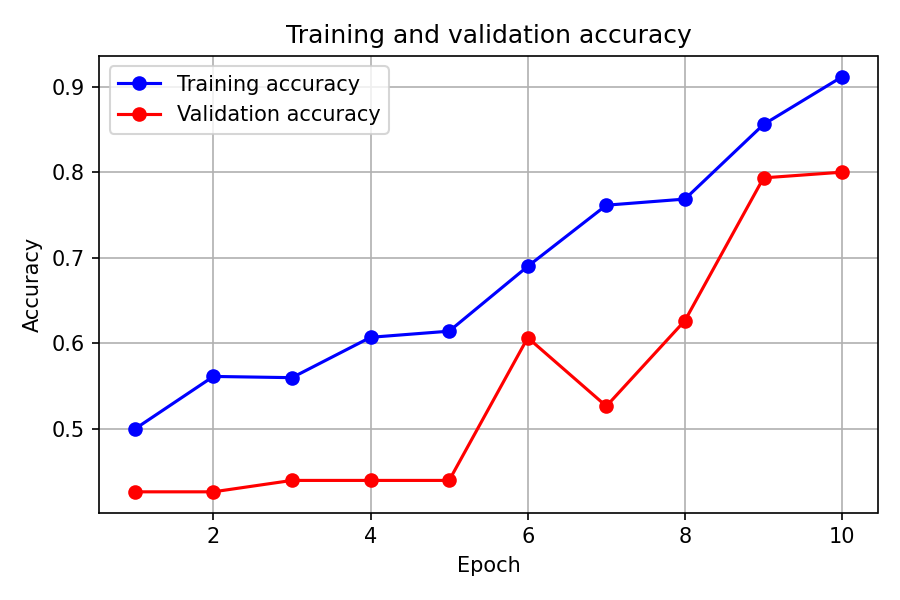
\includegraphics[width=1.0\linewidth]{./images/tanh_accuracy.png}
    \caption{Přesnost pro konfiguraci \texttt{tanh}; výkon je podobný jako u ReLU.\label{fig:tanh-acc}}
\end{figure}

\begin{figure}[ht!]
    \centering
    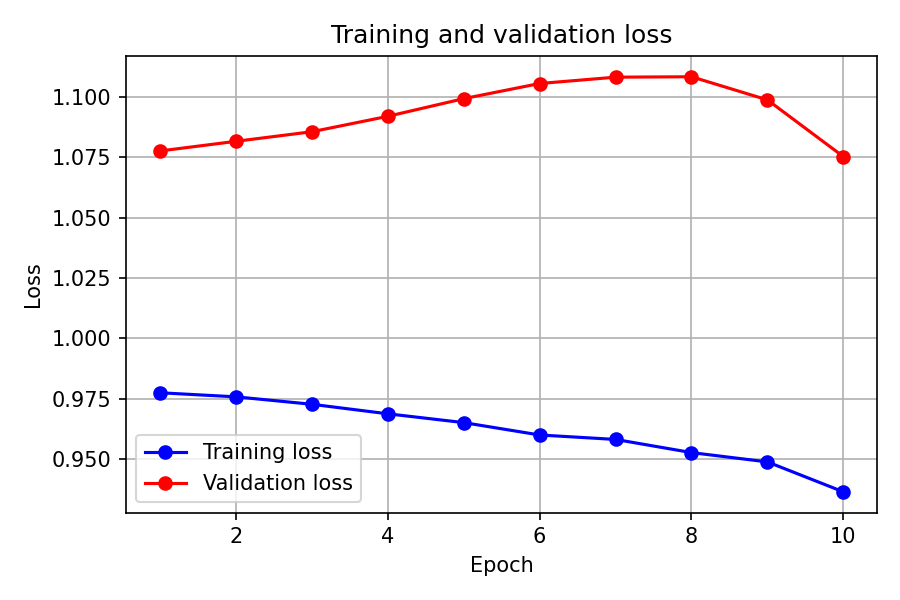
\includegraphics[width=1.0\linewidth]{./images/hinge_loss.png}
    \caption{Ztráta pro konfiguraci \texttt{hinge} s marginovou ztrátou, kde model dosahuje nejhorší generalizace.\label{fig:hinge-loss}}
\end{figure}

\begin{figure}[ht!]
    \centering
    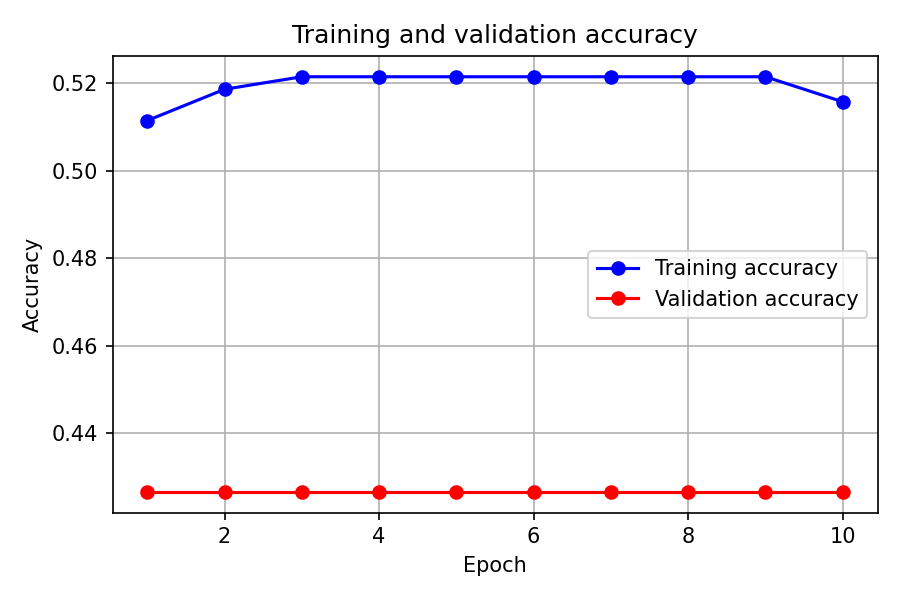
\includegraphics[width=1.0\linewidth]{./images/hinge_accuracy.png}
    \caption{Přesnost pro konfiguraci \texttt{hinge}; výsledky jsou blízké náhodnému hádání.\label{fig:hinge-acc}}
\end{figure}

\begin{figure}[ht!]
    \centering
    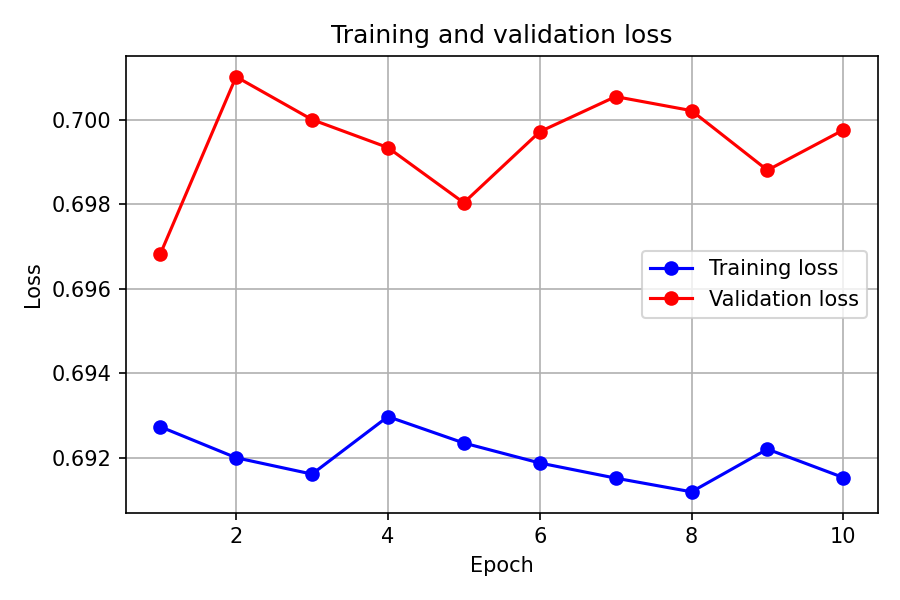
\includegraphics[width=1.0\linewidth]{./images/sgd_loss.png}
    \caption{Průběh ztráty pro konfigurace s optimalizátorem SGD.\label{fig:sgd-loss}}
\end{figure}

\begin{figure}[ht!]
    \centering
    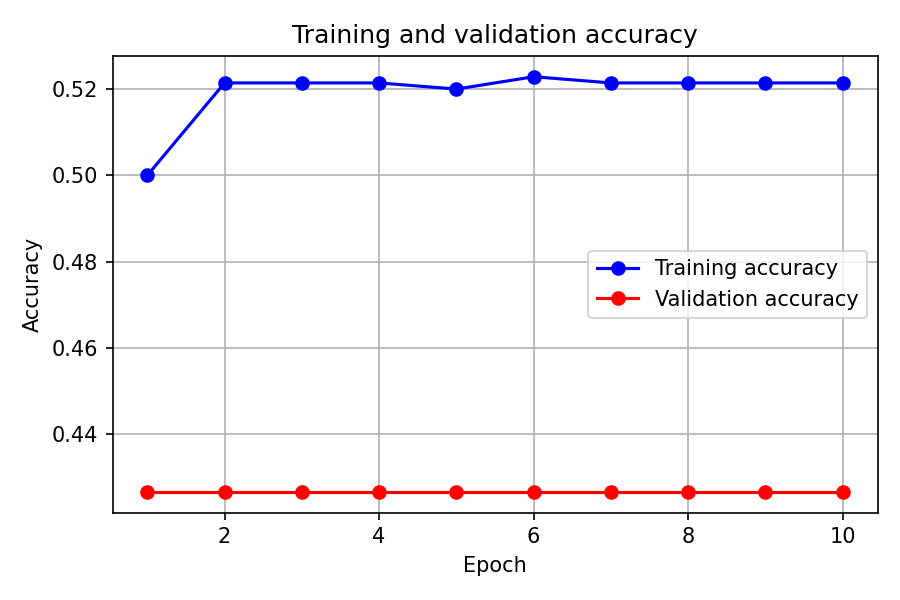
\includegraphics[width=1.0\linewidth]{./images/sgd_accuracy.png}
    \caption{Přesnost pro konfigurace s optimalizátorem SGD.\label{fig:sgd-acc}}
\end{figure}

\begin{figure}[ht!]
    \centering
    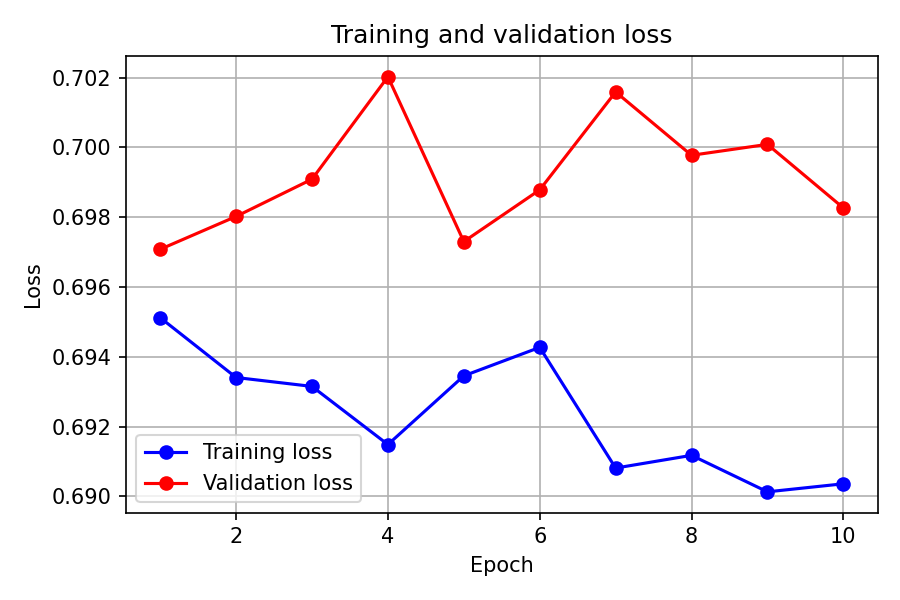
\includegraphics[width=1.0\linewidth]{./images/rmsprop_loss.png}
    \caption{Průběh ztráty pro konfigurace s optimalizátorem RMSprop.\label{fig:rmsprop-loss}}
\end{figure}

\begin{figure}[ht!]
    \centering
    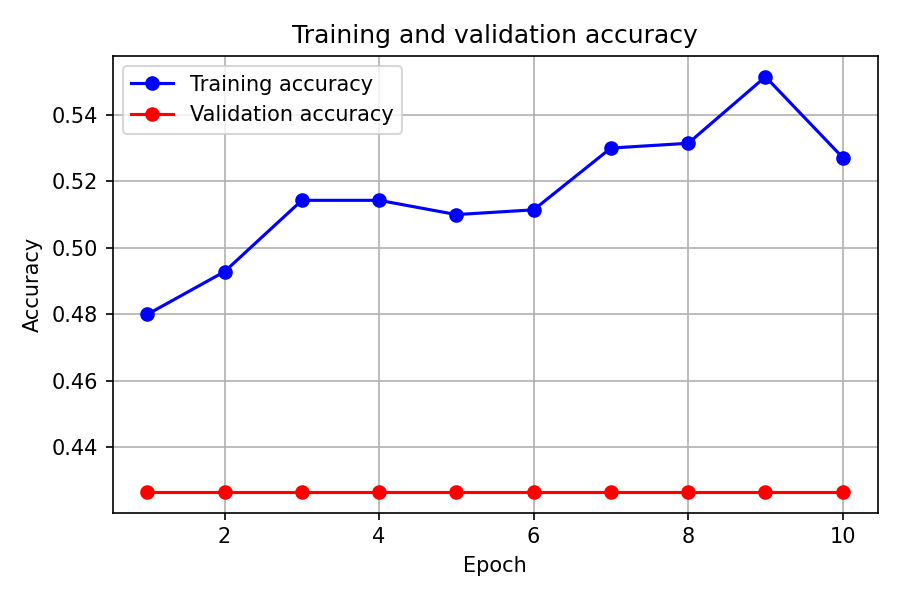
\includegraphics[width=1.0\linewidth]{./images/rmsprop_accuracy.png}
    \caption{Přesnost pro konfigurace s optimalizátorem RMSprop.\label{fig:rmsprop-acc}}
\end{figure}

\end{document}
